\documentclass[a4paper,12pt,UTF8,fontset=none]{ctexart}
\usepackage{geometry} % 页面设置
\usepackage{xeCJK}
\usepackage{enumitem}
\usepackage{xcolor} % Color support for listings
\usepackage{graphicx}
\usepackage{pdfpages}
\usepackage{amssymb} % For join symbol
\usepackage{amsmath}
\usepackage{listings}
\usepackage{longtable}
\usepackage{booktabs} % 添加booktabs宏包以支持三线表
\usepackage{array}      % 列格式控制
\usepackage{caption}    % 表格标题格式
\usepackage{placeins} 
\usepackage{newtxtext,newtxmath}
\usepackage{fontspec}
\usepackage{titlesec}
\usepackage{cleveref}

% 设置英文主字体为 Times New Roman
\setmainfont{Times New Roman}[Path=D:/Program Files/MiKTeX/fonts/custom/, Extension=.otf]

% 设置英文粗体字体为 Times New Roman Bold
\newfontfamily\enboldfont{Times New Roman Bold}[Path=D:/Program Files/MiKTeX/fonts/custom/, Extension=.otf]

% 设置中文正文字体为宋体
\setCJKmainfont{SimSun}[Path=D:/Program Files/MiKTeX/fonts/custom/, Extension=.ttf]

% 设置中文黑体字体
\setCJKfamilyfont{zhhei}{SimHei}[Path=D:/Program Files/MiKTeX/fonts/custom/, Extension=.ttf]
\newcommand{\heiti}{\CJKfamily{zhhei}}


% 自定义编号格式
\renewcommand{\thesection}{\arabic{section}}
\renewcommand{\thesubsection}{\thesection.\arabic{subsection}}
\renewcommand{\thesubsubsection}{\thesubsection.\arabic{subsubsection}}
% 设置标题格式
\titleformat{\section}
  {\centering\heiti\zihao{-3}\enboldfont}{\thesection}{1em}{}
\titleformat{\subsection}
  {\heiti\zihao{4}\enboldfont}{\thesubsection}{1em}{}
\titleformat{\subsubsection}
  {\heiti\zihao{-4}\enboldfont}{\thesubsubsection}{1em}{}



% 设置代码块样式
\lstset{
    basicstyle=\ttfamily,
    columns=fullflexible,
    frame=single,
    breaklines=true,
    postbreak=\mbox{\textcolor{red}{$\hookrightarrow$}\space},
    language=SQL,
    keywordstyle=\color{blue},
    commentstyle=\color{gray},    
    rulecolor=\color{black!30},%边框颜色
    stringstyle=\color{red},
    escapeinside={\%*}{*)},
    showstringspaces=false,
    captionpos=b % 设置标题位置, b表示在底部
}
\geometry{left=2.5cm,right=2.5cm,top=2.5cm,bottom=2.5cm} % 页边距


\begin{document}

% 制作封面页
\begin{titlepage}
    \centering
    \vspace*{\fill}
    {\LARGE\bfseries 数据库系统原理课程\par}
    \vspace{2cm}
    {\Huge\bfseries 查漏补缺\par}
    \vspace{2cm}
    {\Large 烂石\par}
    \vspace{1cm}
    {\large \today \par}
    \vspace{4cm}
    
\includegraphics[width=0.5\textwidth]{static/images/logo.jpg}
    \vspace*{\fill}
    \thispagestyle{empty} % 封面不显示页码
    \newpage
\end{titlepage}
\section{数据库概念}
\subsection{模型概念体系}

\begin{figure}[htbp]
    \centering
    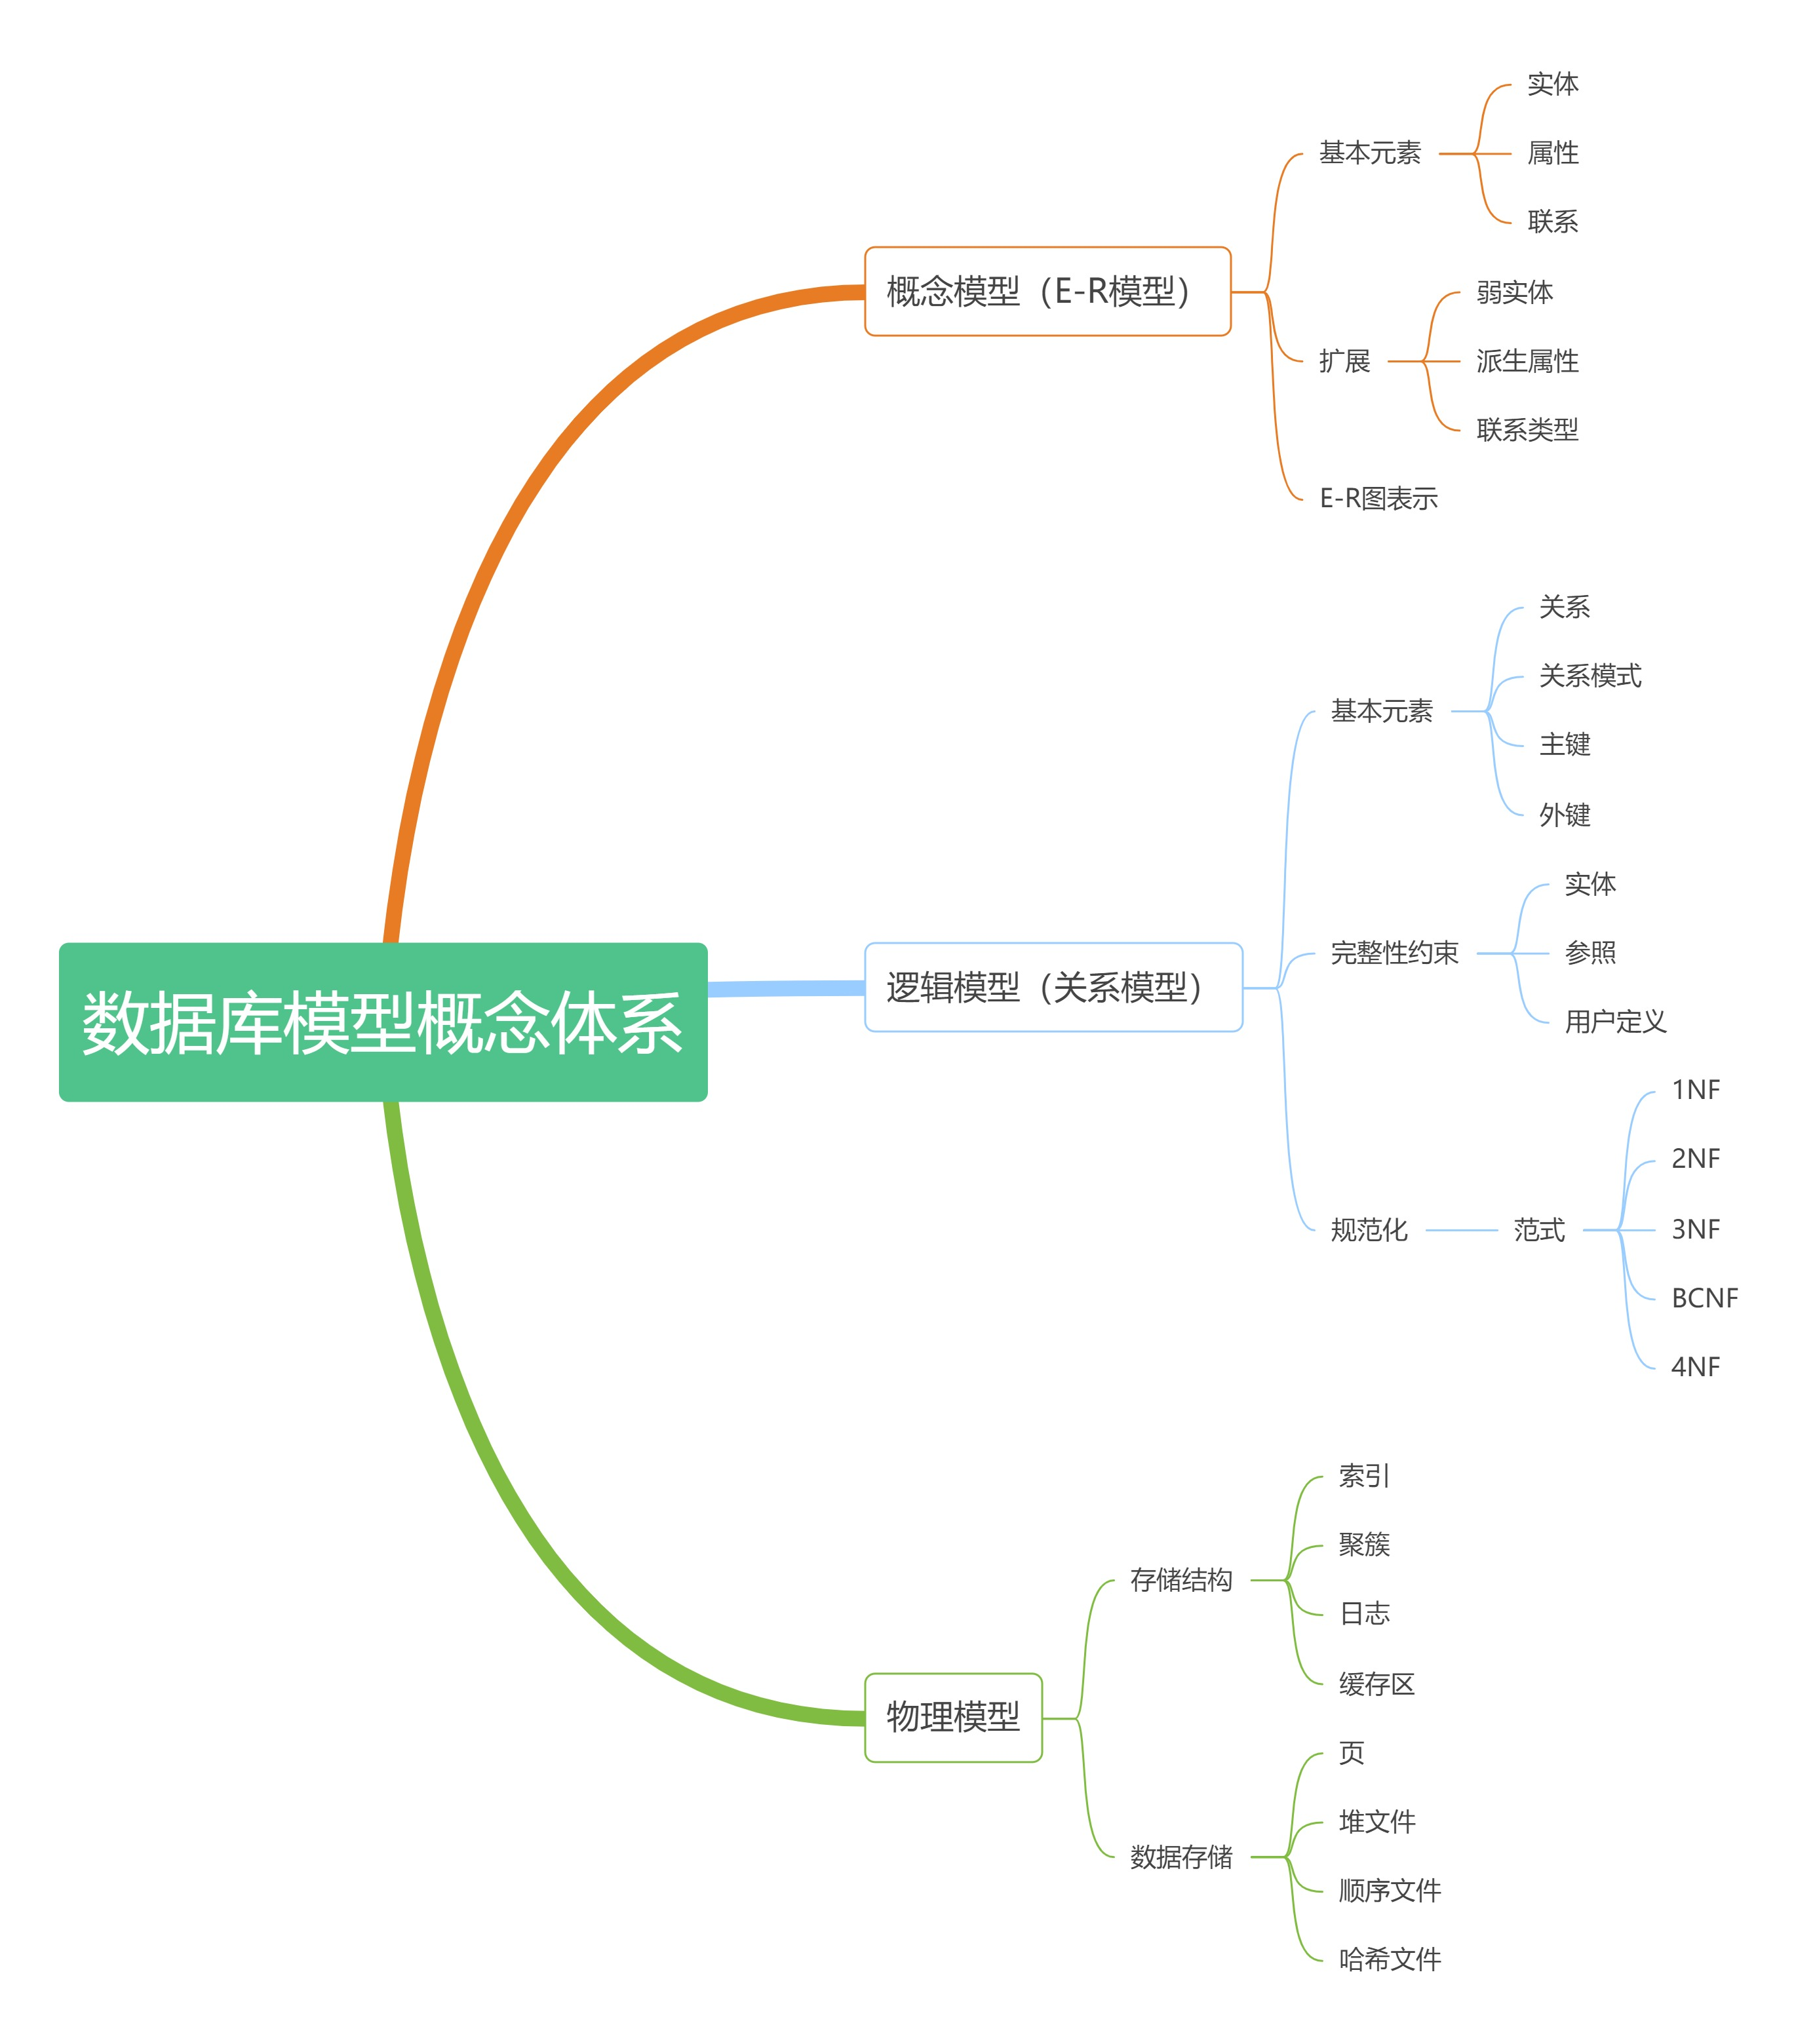
\includegraphics[width=0.8\textwidth]{static/images/数据库模型概念体系.jpg} % 调整宽度和路径
    \caption{数据库模型概念体系图} % 添加标题
    \label{fig:database-model-system} % 可选:添加标签以便引用
\end{figure}
\end{document}